% This file was converted to LaTeX by Writer2LaTeX ver. 1.9.9
% see http://writer2latex.sourceforge.net for more info
\documentclass{article}
\usepackage{calc,amsmath,amssymb,amsfonts}
\usepackage[LGR,T1]{fontenc}
\usepackage[greek,spanish]{babel}
\usepackage{array,supertabular,hhline,graphicx}
\setlength\tabcolsep{1mm}
\renewcommand\arraystretch{1.3}
\newcounter{Figure}
\renewcommand\theFigure{\arabic{Figure}}
\author{Brandon Marquez Salazar}
\date{2026-07-07}
\begin{document}
\clearpage

Particles and Weed into the Swampland: Testing Metaheuristics Ability for Vacua Search in String Theory
Brandon Marquez Salazar1, César Eduardo Damián Ascencio1, Ángel Díaz Pacheco1

1División de Ingenierías Campus Irapuato–Salamanca, Universidad de Guanajuato. Carretera Salamanca - Valle de Santiago
Km. 3.5 + 1.8; Comunidad de Palo Blanco; Salamanca, Guanajuato, México.

b.marquezsalazar@ugto.mx, angel.diaz@ugto.mx, cesar.damian@ugto.mx
Anoymous Author
Abstract

In the fields of String Theory models behave in so very convoluted ways it$\text{\textgreek{’}}$s necessary the use of
metaheuristic approaches to help in the search within the swampland.

Resumen

En el área de la Teoría de Cuerdas, los modelos se comportan de formas tan convulsas que es necesario el uso de
aproximaciones metaheurísticas para apoyar la búsqueda dentro del Swampland.
\_\_\_\_\_\_\_\_\_\_\_\_\_\_\_\_\_\_\_\_\_

Keywords and phrases: String Theory, Swampland, Bio‑Inspired Algorithms, Nature‑Inspired Algorithms, Metaheuristics,
Optimisation, No Free Lunch Theorem.

%
%Revisar qué significa y si se debe conservar, cambiar o retirar.
%Brandon Marquez Salazar
%22 de junio de 2026 16:59
2020 Mathematics Subject Classification: 68N01 

\_\_\_\_\_\_\_\_\_\_\_\_\_\_\_\_\_\_\_\_\_
1 Introduction

There are several problems which can$\text{\textgreek{’}}$t be easily solved by analytical methods nor deterministic
numerical algorithms due to their complexity or it$\text{\textgreek{’}}$s capricious unpredictable behaviour. In the
fields of string theory, mathematical models predicts an extensive amount of possible universe configurations which
may, in most of the cases, not correspond to our universe $\text{\textgreek{—}}$to say, tachyonic, too high or negative
potential. Thus, some approaches in this field often involves artificial intelligence and machine learning approaches
[1], [2]
2 Theoretical Framework and State of the Art

The exploration of the string landscape through computational intelligence has grown steadily over the past decade, with
metaheuristics playing an increasingly central role in navigating the enormous space of possible vacuum configurations.
This section reviews the foundational contributions that establish the context for our proposed benchmark study
comparing Inertica Weight Particle Swarm Optimisation (PSO) [3] and Invasive Weed Optimisation (IWO) \ against
established genetic algorithm (GA) [4], [5], [6] and simulated annealing (SA) [1], [7] baselines.

\subsubsection{2.1 Genetic Algorithms in the String Landscape}
The pioneering work of Abel and Rizos [5] demonstrated that genetic algorithms can efficiently explore the string
landscape in free fermionic models. Despite a search space of astronomical size$\text{\textgreek{—}}$estimated at 251
possibilities$\text{\textgreek{—}}$the GA proved to be orders of magnitude more efficient than random sampling at
locating vacua with specific phenomenological properties. This result was significant because it revealed that the
landscape's structure, though complex, is amenable to evolutionary search, where selection and recombination guide the
population toward promising regions.

Building on this foundation, Damian and Loaiza-Brito [8] implemented a genetic algorithm to search for stable de Sitter
(dS) and anti-de Sitter (AdS) vacua in Type IIB compactifications on six-dimensional tori threaded with standard and
S-dual invariant nongeometric fluxes. Their approach yielded 11 AdS and 7 dS stable vacua, establishing the GA as a
viable tool for exploring flux compactifications. Notably, they observed a consistent mass hierarchy wherein complex
structure moduli were heavier than the Hubble scale, suggesting that Kähler moduli are natural candidates for
small-field inflation. In a companion work [9] Damian extended this analysis to demonstrate that multi-field inflation
driven by the axio-dilaton and Kähler moduli is a viable scenario in all stable dS vacua they reported, with the
inflaton direction approximately orthogonal to the s-goldstino.

\subsubsection[2.2 Machine Learning{}-Enhanced Exploration]{2.2 Machine Learning-Enhanced Exploration}
The synergy between machine learning and metaheuristics has opened new avenues for landscape exploration. Cabo Bizet et
al. combined an artificial neural network (ANN) with a genetic algorithm to classify over sixty thousand flux
configurations in Type IIB compactifications on an isotropic torus. Their supervised learning approach achieved a
classification accuracy of 98.6\%, successfully identifying flux patterns leading to critical points of the scalar
potential. The ANN+GA hybrid proved significantly more efficient than GA alone, reducing computational time while
maintaining solution quality. Critically, their analysis confirmed the refined de Sitter conjecture: no stable dS vacua
were found, and the distribution of critical points satisfied the bound  $\text{min}\nabla i\nabla jV\le -c'V$ \ with 
$c'$ \ of order 1. [2]

\subsubsection{2.3 Torsion Compactifications and the Simulated Annealing Baseline}
A significant advancement came with the work of Damian and Loaiza-Brito [1], who considered Type IIB compactifications
on Kähler manifolds with torsion. By incorporating contributions from the five-form flux and non-BPS D5-branes wrapping
torsional cycles, they constructed an effective scalar potential of the form

\begin{center}
\tablefirsthead{}
\tablehead{}
\tabletail{}
\tablelasttail{}
\begin{supertabular}{m{13.893001cm}m{1.296cm}}
 $V_{\mathit{eff}\text{\hspace{0pt}}}=\mathit{frac}A_{H_3}\text{\hspace{0pt}}\text{\hspace{0pt}}s\tau
^3\text{\hspace{0pt}}+\mathit{frac}A_{F_3}s\tau
^3\text{\hspace{0pt}}\text{\hspace{0pt}}\text{\hspace{0pt}}+\mathit{frac}A_{F_5}\tau
^4\text{\hspace{0pt}}\text{\hspace{0pt}}+\mathit{frac}A_3\text{[D835?][DCDD?]}_3\tau
^3\text{\hspace{0pt}}\text{\hspace{0pt}}+\mathit{frac}A_{\widehat {\mathit{D5}}}\text{\hspace{0pt}}s^{1/2}\tau ^{5/2}$ 
&
(1)\\
\end{supertabular}
\end{center}
where s and $\tau $ are the axio-dilaton and Kähler moduli respectively, and the  $A_i$\hspace{0pt} coefficients
represent flux contributions. This model provided a concrete mechanism for uplifting AdS vacua to dS through non-BPS
states. Implementing a hybrid simulated annealing (SA) and conjugate gradient (CG) algorithm, they reported over 170
stable dS vacua (Damian \& Loaiza-Brito, 2022). Their analysis revealed two essential conditions for stable uplifting:
(1) RR and NS-NS 3-form fluxes must be supported on more than a single cycle, and (2) the number of O3-planes must
satisfy the bound

\begin{center}
\tablefirsthead{}
\tablehead{}
\tabletail{}
\tablelasttail{}
\begin{supertabular}{m{13.893001cm}m{1.296cm}}

$\text{[D835?][DCDD?]}_{\mathit{O3}}\text{\hspace{0pt}}>4\mathit{frac}\sqrt{\text{\hspace{0pt}}A_{H_3}\text{\hspace{0pt}}\text{\hspace{0pt}}A_{F_3}}A_3\text{\hspace{0pt}}\text{\hspace{0pt}}\text{\hspace{0pt}}+2\text{[D835?][DCDD?]}_{\mathit{flux}}\text{\hspace{0pt}}$
 &
(2)\\
\end{supertabular}
\end{center}
\subsubsection{2.4 Gap Identification and Motivation for Extended Benchmarking}
While the works reviewed above have successfully applied GA [2], [8] and SA [1] to specific string compactification
models, the question remains whether other nature-inspired algorithms could achieve even better performance in terms of
convergence speed, solution quality, or the number of vacua discovered. Specifically, no systematic comparison of
different metaheuristic families has been performed on the torsion compactification model defined by Equation (1). The
No Free Lunch theorem [10] reminds us that no single optimisation algorithm is universally superior; performance
depends on the specific properties of the objective function and search space.

Particle Swarm Optimisation (PSO), introduced by Kennedy and Eberhart [11], offers distinct advantages for this problem
class. Unlike GAs, which rely on selection, crossover, and mutation operators, PSO employs a swarm of particles that
move through the search space following social and cognitive components. Each particle adjusts its position based on
its own best-known position and the swarm's best-known position, enabling efficient exploration of the landscape. The
algorithm's simplicity, few hyperparameters, and inherent parallelism make it particularly attractive for
high-dimensional optimisation problems.

Invasive Weed Optimisation (IWO), proposed by Mehrabian and Lucas [12], presents an alternative paradigm inspired by the
colonising behaviour of weeds. Seeds are randomly distributed over the search space, and fitter individuals produce
more seeds, with the standard deviation of seed dispersion decreasing over generations. This mechanism provides a
natural balance between exploration (wide seed dispersion in early generations) and exploitation (local search in later
generations). IWO has demonstrated superior performance in various engineering optimisation problems, though its
application to string theory vacuum searches remains entirely unexplored.

The present work addresses this gap by proposing a comprehensive benchmark study comparing PSO and IWO against the
established GA and SA baselines in the torsion compactification model of Damian and Loaiza-Brito [1]. By evaluating
these algorithms across multiple moduli configurations and performance metrics$\text{\textgreek{—}}$including
convergence speed, solution quality, stability ratios, and the number of novel vacua discovered$\text{\textgreek{—}}$we
aim to establish whether alternative metaheuristic families can further improve the exploration of the string landscape
and provide a robust computational benchmark for future research.

3 Methods and Materials
The model to optimise is the effective potential (1) showed in section 2.3 whose definition can be found in the work of
Damian and Loaiza-Brito [1]. However as previously shown, the use of the four descriptors demonstrated better results
compared with other approaches, nevertheless each one of the descriptors were symbolically obtained from the original
potential. This was done as well in this work with two purposes: a) to keep the new code the more similar possible to
the original, and b) to have the highest precision possible in the search.

The original code written in Wolfram Mathematica was implemented in this work as a python module for this language
having spread with a large AI/ML community due to the benefit of being a free open source language. This modular
approach permitted a) while it could be separated in different sections. The project is currently powered by sympy,
cupy/numpy and mealpy since sympy can handle and lambdify any symbolic approach, mealpy provides the largest collection
of metaheuristics which is important for this benchmark researches, and cupy offers GPU acceleration support for the
fitness function implemented in sympy.

\subsubsection[3.1 Fitness function wall{}-clock test]{3.1 Fitness function wall-clock test}
A wall-clock was done before constructing the grid since any highly complex function is potentially expensive in
computational terms. The results of the wall-clock are shown in the table 1.

\begin{center}
\topcaption[Results of wall{}-clock test for the fitness function.]{Results of wall-clock test for the fitness
function.}
\tablefirsthead{}
\tablehead{}
\tabletail{}
\tablelasttail{}
\begin{supertabular}{m{3.6959999cm}m{3.6959999cm}m{3.6959999cm}m{3.698cm}}
\hline
 $N$  &
 $t$  &
 $\bar t$ \ in seconds &
 $t^{-1}$ \\\hline
1 &
0.0012930000 &
1.29E-03 &
773.42\\
2 &
0.0023550000 &
1.18E-03 &
849.25\\
3 &
0.0034990000 &
1.17E-03 &
857.33\\
7 &
0.0082160000 &
1.17E-03 &
851.98\\
11 &
0.0133640000 &
1.214935e-03 &
823.09\\
10 &
0.0114730000 &
1.15E-03 &
871.58\\
20 &
0.0240690000 &
1.20E-03 &
830.93\\
30 &
0.0352240000 &
1.17E-03 &
851.69\\
70 &
0.0821420000 &
1.17E-03 &
852.18\\
110 &
0.1285840000 &
1.168944e-03 &
855.47\\
100 &
0.1172440000 &
1.17E-03 &
852.93\\
200 &
0.2352520000 &
1.18E-03 &
850.15\\
300 &
0.3525780000 &
1.18E-03 &
850.88\\
700 &
0.8269840000 &
1.18E-03 &
846.45\\
1100 &
1.2978350000 &
1.18E-03 &
847.57\\
2000 &
2.3604520000 &
1.18E-03 &
847.3\\
3000 &
3.5257810000 &
1.18E-03 &
850.88\\
7000 &
8.2698410000 &
1.18E-03 &
846.45\\
11000 &
12.9783510000 &
1.18E-03 &
847.57\\
20000 &
23.6045190000 &
1.18E-03 &
847.3\\
30000 &
35.2578080000 &
1.18E-03 &
850.88\\
70000 &
82.6984450000 &
1.18E-03 &
846.45\\
110000 &
129.7835390000 &
1.179850e-03 &
847.57\\\hline
\end{supertabular}
\end{center}
After this, there were run 2 more tests and then performed a linear regression comparing  $N$  to  $t$  \ and  $N$  to 
$t^{-1}$  for each of the 3 tests, getting the plots obtained at figure 1.


\bigskip

Figure \stepcounter{Figure}{\theFigure}: Linear regressions performed. Left plots show the linear regression comparing 
$N$  against  $t$ . Right plots show the linear regression comparing  $N$  against  $t^{-1}$ . The plots shows scatter
for the points given by the wall-clock test. And the 3 regressions performed.

\begin{center}
\tablefirsthead{}
\tablehead{}
\tabletail{}
\tablelasttail{}
\begin{supertabular}{ll}
 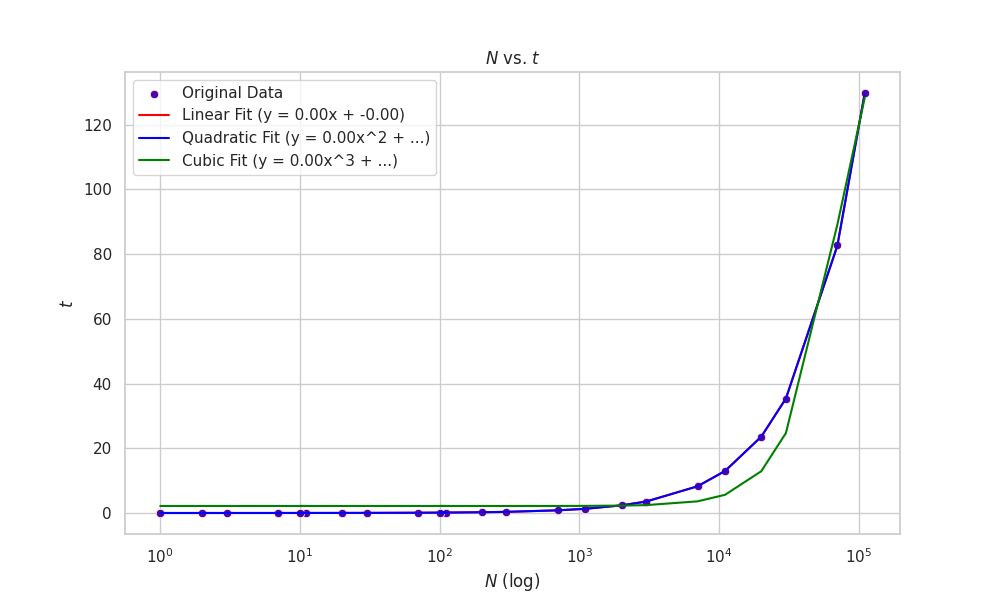
\includegraphics[width=7.601cm,height=5.106cm]{Genes20Particles20and20Weed20into20the20Swamplandodt-img001.png}  & 
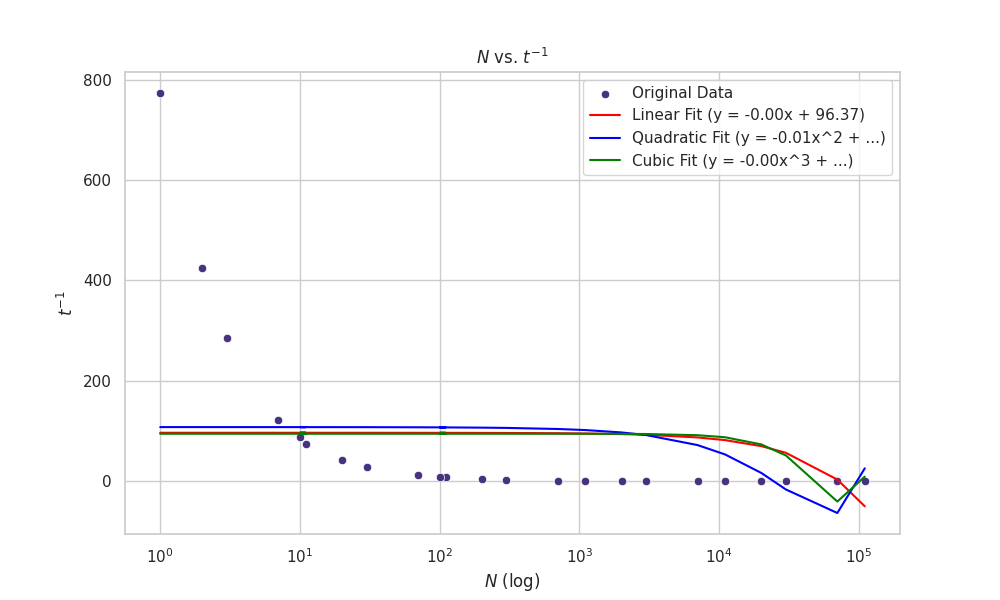
\includegraphics[width=7.601cm,height=5.099cm]{Genes20Particles20and20Weed20into20the20Swamplandodt-img002.png} \\
 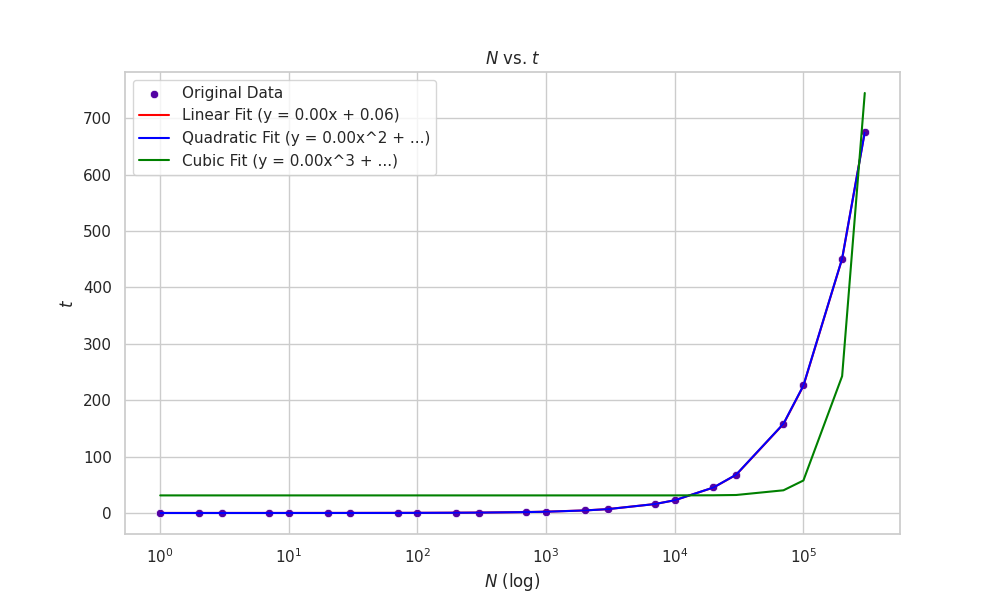
\includegraphics[width=7.601cm,height=5.106cm]{Genes20Particles20and20Weed20into20the20Swamplandodt-img003.png}  & 
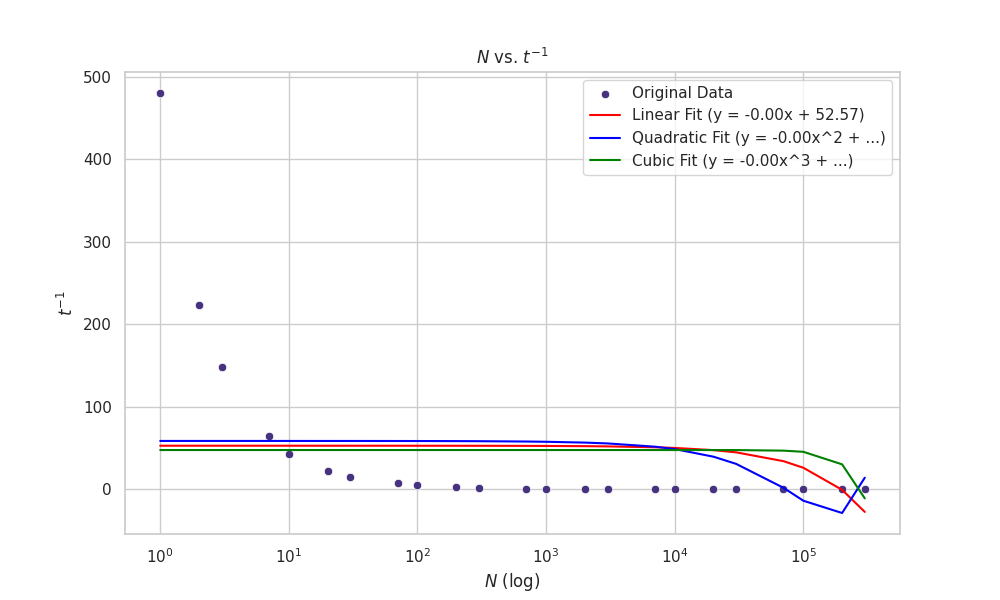
\includegraphics[width=7.601cm,height=5.099cm]{Genes20Particles20and20Weed20into20the20Swamplandodt-img004.png} \\
 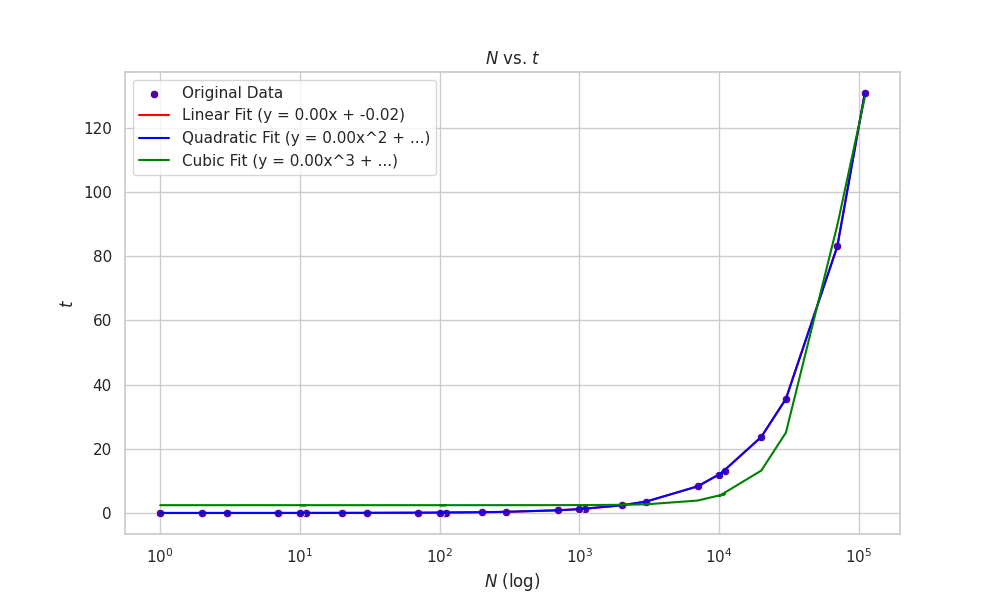
\includegraphics[width=7.601cm,height=5.099cm]{Genes20Particles20and20Weed20into20the20Swamplandodt-img005.png}  & 
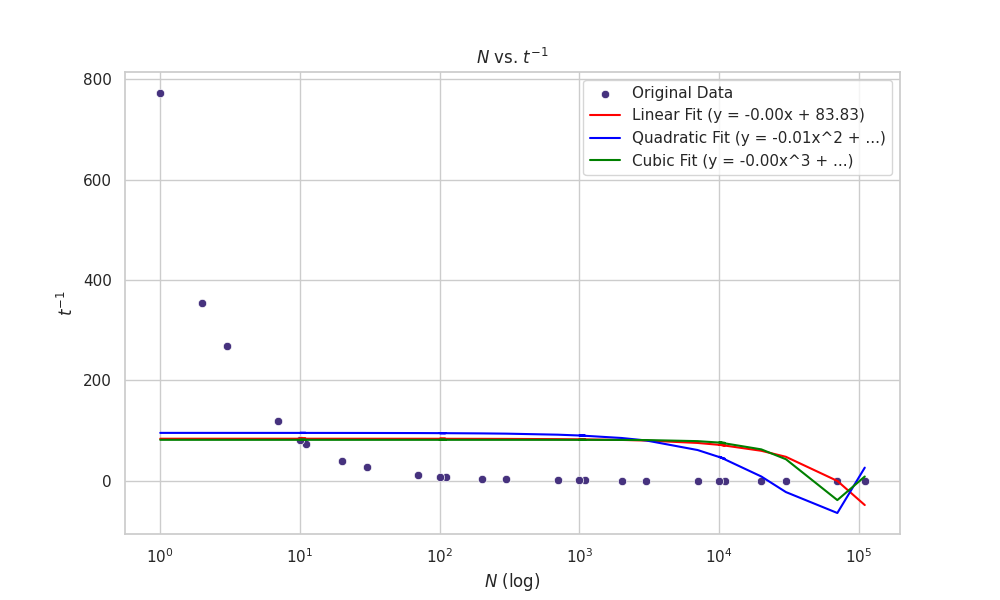
\includegraphics[width=7.65cm,height=5.14cm]{Genes20Particles20and20Weed20into20the20Swamplandodt-img006.png} \\
\end{supertabular}
\end{center}
As it can be noted, the number of iterations per second tends to decrease and stabilise in a range comprehending from
420 (lowest) to 850 (highest) with the increment of  $N$ \ while the time to complete all the iterations increases in a
presumably linear way. This helps us to visualise the temporal cost of within any optimiser algorithm, considering that
each algorithm will sum its computational and temporal costs of the operations set.

\subsubsection{3.2 GA, IWO and PSO implementation}
PSO and IWO were implemented into a grid following mealpy$\text{\textgreek{’}}$s implementation default operators and
structure for no algorithm is proved to outperform in every possible problem [10]$\text{\textgreek{—}}$it is assumed
that this problem corresponds to a new class where it is needed to perform a search from scratch.

IWO defaults taken. a

GA defaults taken. a

\subsubsection{3.3 Criteria and statistical analysis}
The optimisation focuses mainly on minimal points which correspond to low energy critical points for the potential, this
point is later evaluated so it can be classified as de Sitter or Anti de Sitter and as Stable or Tachyonic. The search
for stable/metastable vacua is of special interest in this line of research [9], being important that any point assures
the minimal potential possible$\text{\textgreek{—}}$assuming the precision loss of the optimiser.

Said that, the main criteria results to be the ratios of stable vacua found and the potential statistics such as mean,
standard deviation, skew and visual violin plots.
\subsection{4 Experiments and Results}
Due to high nonlinearity of the model, the grid granularity was high in a large range of variations leading to at least
8K different combinations. Last experiments demonstrated to , the grid was built using 10 configurations per optimiser
within a high granularity combination of hyperparameters$\text{\textgreek{—}}$expect not much variation. All the 10
configurations will be tested using graphic hardware acceleration by cupy.

\subsubsection{4.1 Search conditions}
The search was performed using preconfigured moduli pairs for the search being strictly on coefficients, repeating the
optimisation 100 times per pair across 87 different pairs. These pairs were obtained from optimisation results of [1]. 
5 Conclusions
6 Discussion
References

[1]\ \ C. Damian and O. Loaiza-Brito, “Metastable vacua from torsion and machine learning,” Eur. Phys. J. C, vol. 82,
no. 12, Dec. 2022, doi: 10.1140/epjc/s10052-022-11118-x.

[2]\ \ N. C. Bizet, C. Damian, O. Loaiza-Brito, D. K. Mayorga Peña, and J. A. Montañez-Barrera, “Testing swampland
conjectures with machine learning,” Eur. Phys. J. C, vol. 80, no. 8, Aug. 2020, doi: 10.1140/epjc/s10052-020-8332-9.

[3]\ \ Z. Qin, F. Yu, Z. Shi, and Y. Wang, “Adaptive Inertia Weight Particle Swarm Optimization,” in Artificial
Intelligence and Soft Computing – ICAISC 2006, Springer Berlin Heidelberg, 2006, pp. 450–459. doi:
10.1007/11785231\_48.

[4]\ \ J. H. Holland, “Genetic Algorithms,” Sci. Am., vol. 267, no. 1, pp. 66–72, Jul. 1992, doi:
10.1038/scientificamerican0792-66.

[5]\ \ S. Abel and J. Rizos, “Genetic algorithms and the search for viable string vacua,” J. High Energy Phys., vol.
2014, no. 8, Aug. 2014, doi: 10.1007/jhep08(2014)010.

[6]\ \ A. Cole, S. Krippendorf, A. Schachner, and G. Shiu, “Probing the Structure of String Theory Vacua with Genetic
Algorithms and Reinforcement Learning,” 2021.

[7]\ \ S. Kirkpatrick, C. D. Gelatt, and M. P. Vecchi, “Optimization by Simulated Annealing,” Science, vol. 220, no.
4598, pp. 671–680, May 1983, doi: 10.1126/science.220.4598.671.

[8]\ \ C. Damian and O. Loaiza-Brito, “More stable de Sitter vacua from [D835?][DCE2?]-dual nongeometric fluxes,” Phys.
Rev. D, vol. 88, no. 4, Aug. 2013, doi: 10.1103/physrevd.88.046008.

[9]\ \ C. Damian, L. R. Díaz-Barrón, O. Loaiza-Brito, and M. Sabido, “Slow-roll inflation in non-geometric flux
compactification,” J. High Energy Phys., vol. 2013, no. 6, Jun. 2013, doi: 10.1007/jhep06(2013)109.

[10]\ \ D. H. Wolpert and W. G. Macready, “No free lunch theorems for optimization,” IEEE Trans. Evol. Comput., vol. 1,
no. 1, pp. 67–82, Apr. 1997, doi: 10.1109/4235.585893.

[11]\ \ J. Kennedy and R. Eberhart, “Particle swarm optimization,” in Proceedings of ICNN$\text{\textgreek{’}}$95 -
International Conference on Neural Networks, in ICNN-95, vol. 4. IEEE, pp. 1942–1948. doi: 10.1109/icnn.1995.488968.

[12]\ \ A. R. Mehrabian and C. Lucas, “A novel numerical optimization algorithm inspired from weed colonization,” Ecol.
Inform., vol. 1, no. 4, pp. 355–366, Dec. 2006, doi: 10.1016/j.ecoinf.2006.07.003.
\end{document}
